\subsection{Canales de decaimiento y tasas de ramificación}

\noindent Los canales de desintegración (\textit{decaimiento}) son los posibles cambios que puede tener una partícula a medida que se desintegra, estos se muestran en la figura \ref{channels}.

\begin{figure*}%[H]
    \begin{center}
        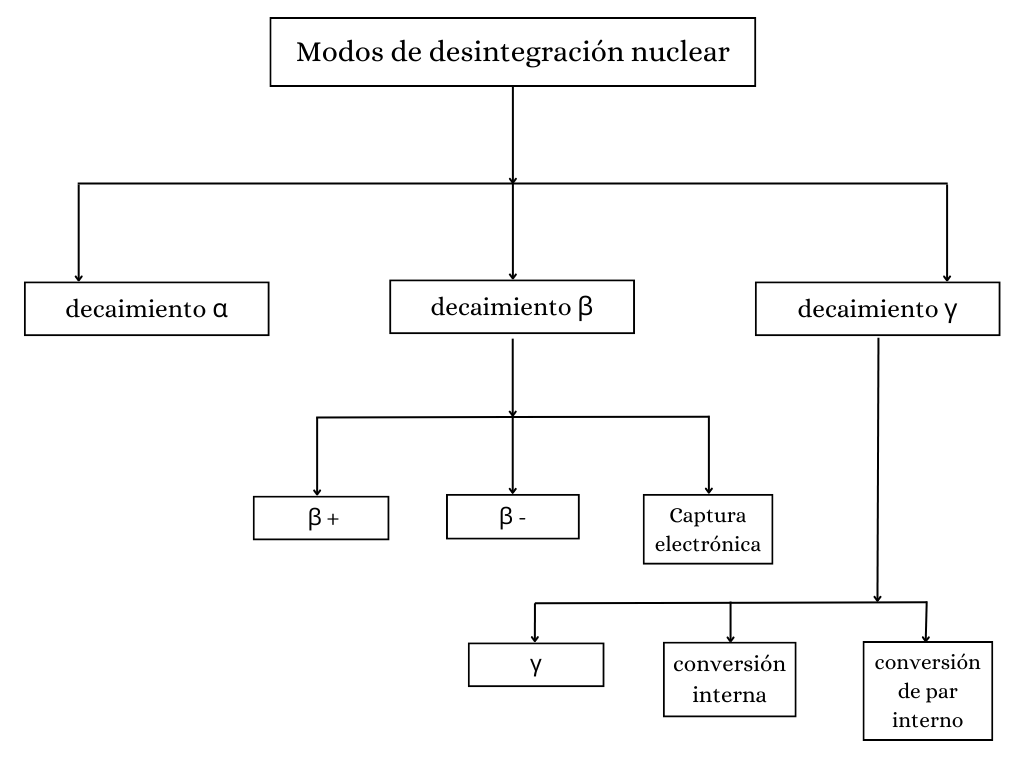
\includegraphics[scale=0.5]{imagenes/decay.png}
        \caption{Canales de desintegración para un radionúclido.}\label{channels}
    \end{center}
\end{figure*}

\noindent Según el tipo de átomo en cuestión, la desintegración radiactiva se produce a través de la emisión de diferentes tipos de radiaciones. Los principales son: 

\begin{itemize}
	\item Radiación alfa ($\alpha $):  la partícula emitida corresponde a un núcleo del elemento químico de helio. La masa del nuevo núcleo disminuye en cuatro unidades, con relación al núcleo inicial. Así, por ejemplo, cuando el átomo de uranio-238 emite una partícula alfa, se transforma en torio-234. La radiación alfa puede recorrer una distancia de apenas unos cuantos centímetros en el aire y puede ser detenida por una simple hoja de papel \cite{Krane.1987}.
	
	\item Radiación beta ($\beta $): la partícula emitida es un electrón. La masa del núcleo atómico formado no cambia con la transformación de un neutrón en un protón. Un neutrino (partícula elemental de carga cero y de masa extremadamente pequeña) se lleva la energía complementaría liberada en la transformación. La radiación beta puede recorrer una distancia de unos cuantos metros en el aire, y puede ser detenida con una placa de vidrio o de madera \cite{Krane.1987}. 
	
	\item Radiación gamma ($\gamma $): es un tipo de radiación electromagnética que transporta el exceso de energía de un núcleo inestable. La radiación gamma acompaña a las transformaciones radiactivas alfa y beta, y tiene un fuerte poder penetrante. Puede recorrer cientos de metros en el aire y se requiere de espesores importantes de plomo o cemento para detenerla \cite{Krane.1987}.
\end{itemize}

Los diversos modos de desintegración de un núcleo radiactivo son:

\begin{itemize}
	\item Decaimiento Alfa:
	
	En este proceso, el núcleo padre se desintegra para dar un núcleo hijo y una partícula $\alpha$ ($^{4} He$). El número de masa del núcleo hijo disminuye en cuatro unidades y el número atómico disminuye en dos unidades. Un ejemplo típico de este modo de caída es: 
	\begin{equation}
		^{238} _{92} U \longrightarrow \ ^{238} _{92} Th + ^{4} _{2} He
	\end{equation}
	
	\item Decaimiento Beta:
	
	En este proceso, el núcleo padre se desintegra para dar un núcleo hijo y una partícula $\beta $. Como se muestra en la figura 2, la desintegración $\beta $ se clasifica en tres categorías: 
	
    %	\begin{itemize}
    		\paragraph{Emisión de electrones o desintegración $\beta ^{-}$}: aquí, el núcleo padre se desintegra para dar un núcleo hijo, una partícula a $\beta ^{-}$ (o un electrón) y una nueva partícula llamada antineutrino. El número de masa del núcleo hijo permanece igual y el número atómico aumenta por una unidad. Un ejemplo es:
    	\begin{equation}
    		^{14} _{6} C \longrightarrow \ ^{14} _{7} N + \beta ^{-} + \bar{\nu }
    	\end{equation}
    	
    	\paragraph{Emisión de positrones o decaimiento $\beta ^{+}$}: en este proceso, el núcleo padre se desintegra para dar un núcleo hijo, una partícula $\beta ^{+}$ (o un positrón) y una nueva partícula llamada neutrino. El número de masa del núcleo hijo permanece igual y el número atómico disminuye en una unidad. Un ejemplo es:
    
    	\begin{equation}
    		^{22} _{11} Na \longrightarrow \ ^{22} _{10} Ne + \beta ^{+} + \nu 
    	\end{equation}
    	
    	\paragraph{Captura de electrones}: aquí el núcleo padre captura uno de los electrones orbitales con la emisión de un neutrino (n). El número de masa del núcleo hijo permanece igual y el número atómico disminuye en una unidad. Por ejemplo: 
    	
    	\begin{equation}
    		^{54} _{25} Mn + \beta ^{-}  \longrightarrow \  ^{54} _{24} Cr + \nu 
    	\end{equation}
    	
 %   	\end{itemize}
 
	\item Decaimiento Gamma:
	
	\noindent Si la energía de excitación disponible con un núcleo no es suficiente para la emisión de partículas, pierde su energía siguiendo tres procesos, como se muestra en la figura [\ref{channels}]. 
	
        \paragraph{Desintegración gamma}: las desintegraciones alfa y beta de un núcleo radiactivo suelen dejar al núcleo hijo en un estado excitado. Si la energía de excitación disponible con el núcleo hijo no es suficiente para una mayor emisión de partículas, pierde su energía al emitir radiaciones electromagnéticas, también conocidas como rayos g. La masa y la carga del núcleo hijo siguen siendo las mismas que antes de la emisión de rayos g. Un ejemplo es: 
    		\begin{equation}
    		^{137} _{56} Ba^{*} \longrightarrow \ ^{137} _{56} Ba + \gamma  
    		\end{equation}
    		El asterisco (*) en Ba indica que está en estado excitado o metaestable.
    		
    		\paragraph{Conversión interna}: en el proceso de conversión interna, un núcleo excitado en lugar de emitir rayos g transfiere directamente su energía de excitación a uno de los electrones orbitales y el electrón orbital es expulsado como electrón de conversión. La masa y la carga del núcleo hijo siguen siendo las mismas que antes de la emisión del electrón orbital. Esto es así porque se expulsa un electrón de las órbitas electrónicas.
    		\paragraph{Conversión de par interno}: si la energía de excitación del núcleo $>$ 1.022 MeV, el núcleo puede des-excitarse emitiendo directamente un par de electrones y positrones en su propio campo de Coulomb. Este proceso se conoce como conversión de pares internos \cite{Podgorsak.2016}.
\end{itemize}


\subsection{Probabilidades de decaimiento}

\noindent Las leyes de la desintegración radiactiva son: 
\begin{enumerate}
    \item Existe la misma probabilidad de que todos los núcleos de un elemento radiactivo se desintegran. 
 	
    \item La tasa de desintegración espontánea de un elemento radiactivo es proporcional al número de núcleos presentes en ese momento \cite{Krane.1987}.
 	
\end{enumerate}

\noindent Matemáticamente, se puede escribir como: 

\begin{equation}
    \frac{dN}{dt} \propto N
\end{equation}

\noindent donde N es el número de átomos presentes en el tiempo t. Eliminando el signo de proporcionalidad, obtenemos: 

\begin{equation}
\frac{dN}{dt} = -\lambda N\label{ecuaciondiferencialN}
\end{equation} 

\noindent Donde $\lambda $ es una constante de proporcionalidad y se conoce como constante de decaimiento del elemento. El signo negativo indica que a medida que t aumenta, N disminuye. Reescribiendo la ecuación \ref{ecuaciondiferencialN} como: 

\begin{equation}
\frac{dN}{N} = -\lambda dt
\end{equation} 

\noindent Integrando ambos lados tenemos: 

\begin{equation}
ln( \lambda ) = -\lambda t + C\label{ecuacionlambda}
\end{equation}

\noindent donde C es una constante de integración y se evalúa por el hecho de que en t = 0, el número de átomos del elemento radiactivo es $N_0$. Usando esta condición, obtenemos: 

\begin{equation}
    C = ln (N_0)
\end{equation}

\noindent Sustituyendo este valor de C en la ecuación \ref{ecuacionlambda}: 

\begin{equation}
    ln\left( \frac{N}{N_0} \right) = - \lambda t 
\end{equation}

\noindent Con esto tenemos que: 

\begin{equation}
    N = N_{0} e^{ - \lambda t }
\end{equation}

\noindent La naturaleza exponencial de esta ecuación muestra que se necesita un tiempo infinito para que todo el material radiactivo se desintegre. N versus t se ha representado gráficamente para $ ^{24} Na$ ($t_{1/2} = 15h$) en la figura \ref{decaimientodelsodio24}. Una gráfica de $log(N)$ frente a $t$ sería una línea recta.

\begin{figure*}
    \begin{center}
        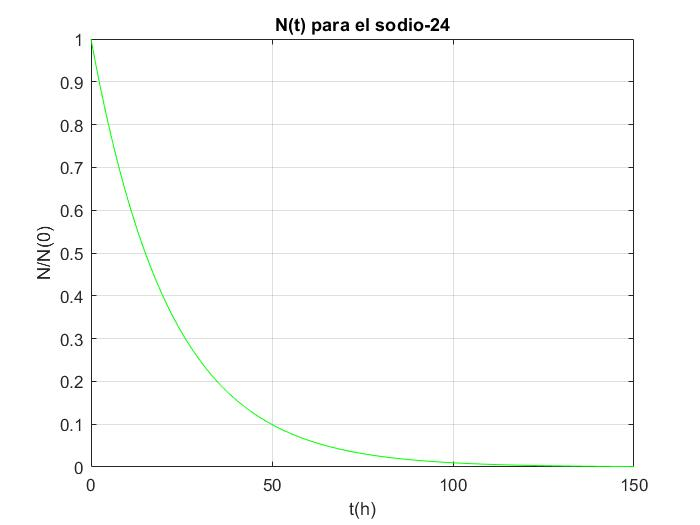
\includegraphics[scale=0.5]{imagenes/decaimiento_sodio_24.jpg}
        \caption{Gráfica del decaimiento exponencial del sodio-24 en en un intervalo de 150 horas.}
        \label{decaimientodelsodio24}
    \end{center}
\end{figure*}

\subsection{Desintegración en cadena}


\subsection{Ecuaciones de Bateman}

\noindent Las ecuaciones de Bateman son un sistema de ecuaciones diferenciales ordinarias propuestas por el matemático británico Harry Bateman en 1910 para generalizar las cadenas de desintegración del tipo $Padre\rightarrow Hijo \rightarrow Nieto$ \cite{Podgorsak.2016}.

\noindent Debido a que la cantidad de núcleos que participan en el proceso de desintegración es tan grande, podemos suponer que la función $N=N(t)$ que da el número de núcleos en un tiempo $t$ es una función continua, no discreta. De esta manera, es posible aplicar sobre ella las reglas de cálculo como ya las conocemos \cite{Podgorsak.2016}. 

\noindent Siguiendo a \textit{Podgorsak} en \cite{Podgorsak.2016}, tenemos que la cadena de desintegración descrita en el modelo de Bateman comprende las siguientes condiciones iniciales:

\begin{equation}
    \eval{N_1(t)}_{t=0}=N_1(0)\neq 0,\label{condicioninicialpadre}
\end{equation}
\begin{equation}
    N_2(0)=N_3(0)=...=N_i(0)=0, \label{condicioninicialproductos}
\end{equation}

\noindent como conveniencia para futuras referencias llamaremos a la ecuación \ref{condicioninicialpadre} \textit{condición inicial del núcleo padre} y a \ref{condicioninicialproductos}, \textit{condición inicial de los productos}. 

\noindent El significado o la implicación de las ecuaciones \ref{condicioninicialpadre} y \ref{condicioninicialproductos} es que, en un tiempo inicial, $t=0$, únicamente disponemos de los núcleos de la muestra padre para desintegración nuclear, mientras que los productos de su fisión permanecen inexistentes. Es solo hasta que el padre ha decaído que comenzamos a ver valores de $N$ distintos de cero para los elementos resultantes de la fisión. 

\noindent El número de núcleos disponibles en un tiempo $t$ para el k-ésimo producto de fisión viene dado por:

\begin{equation}
        N_k(t)=N_1(0) e^{-\lambda_1 t}+C_2 e^{-\lambda_2 t}+...+C_k e^{-\lambda_k t} \label{iesimonucleo}
\end{equation}

\noindent Donde $N_1^{(0)}$ es el número inicial de núcleos de la muestra radiactiva. Para los valores numéricos de los coeficientes $C_k$ de Bateman, \textit{Flanagan y Senftle} en \cite{Flanagan1954} ofrecen tablas completas de los términos que involucran.

En general, \cite{Loch.2013} ofrece una generalización más compacta válida para cualquier núcleo en la secuencia:

\begin{equation}
        N_m(t)=N_1^{(0)} \prod_{k=1}^{m-1}\lambda_k\sum_{j=1}^{m}\left(\frac{e^{\lambda_j t}}{\prod\limits_{p=1, p\neq j}^{m}\left(\lambda_p-\lambda_j\right)}\right) \label{batemangeneral}
\end{equation}

\noindent De acuerdo con \textit{Pratiwi et al} en \cite{Pratiwi.2021}, Bateman habría resuelto sus ecuaciones con transformadas de Laplace, y este método sería efectivo para sistemas lineales \textit{bien portados}, pero en el caso de reacciones en cadena con bifurcaciones en los productos de desintegración sumado a constantes de desintegración diferentes para cada producto, el sistema requiere de un tratamiento matricial numérico. 

En la sección \ref{actinidoserie} se desarrolla el esquema matricial en el caso particular para la cadena del uranio-235. 